

\section{Primitive Concepts}
\label{sec:primitive}
Primitive concepts with a class taxonomy are expected to describe every item and user need in e-commerce accurately and comprehensively.
They are the fundamental building blocks for understanding high-level shopping needs of our customers.
In this section, we mainly introduce how we mine these raw primitive concepts (can be seen as vocabulary) and then organize them into the hierarchical structure.


\subsection{Vocabulary Mining}
\label{sec:mining}
There are two ways of enlarging the size of primitive concepts once the taxonomy is defined.
The first one is to incorporate existing knowledge from multiple sources through ontology matching.
In practice, we mainly adopt rule-based matching algorithms, together with human efforts to manually align the taxonomy of each data source. Details will not be introduced in this paper.

The second one is to mine new concepts from large-scale text corpus generated in the domain of e-commerce such as search queries, product titles, user-written reviews and shopping guides.
Mining new concepts of specific classes can be formulated as \textit{sequence labeling} task,
where the input is a sequence of words and the output is a sequence of predefined labels.
However, the hierarchical structure of our taxonomy is too complicated for this task, 
so we only use the $20$ first-level classes as labels in practice.

\begin{figure}[th]
	\centering
	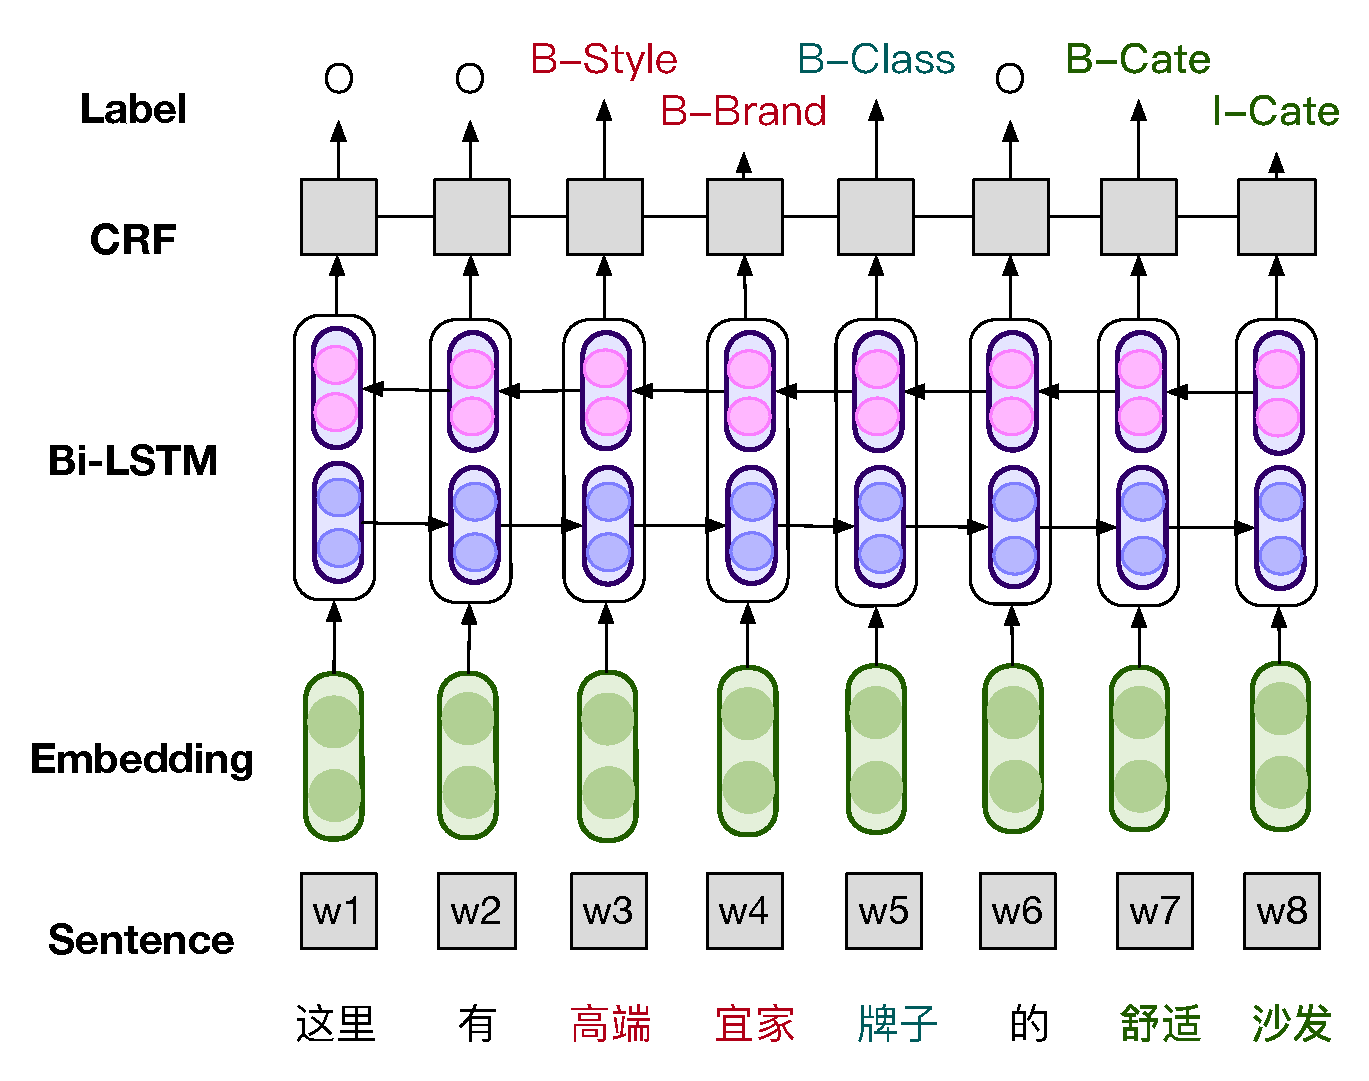
\epsfig{file=figures/bilstm_crf.eps, width=0.85\columnwidth}
	\caption{Principle architecture of a BiLSTM-CRF model
	}
	\label{fig:bilstm_crf}
\end{figure}


\figref{fig:bilstm_crf} shows the principle architecture of a BiLSTM-CRF model,
which is the state-of-the-art model for various sequence labeling tasks \cite{huang2015bidirectional,reimers2017optimal}.
BiLSTM-CRF model consists of a BiLSTM layer and a CRF layer, 
where BiLSTM (Bidirectional-LSTM) enables the
hidden states to capture both historical and future
context information of the words and 
CRF (Conditional Random Field) considers the correlations
between the current label and neighboring
labels.
%Mathematically, the input of this BiLSTM layer
%is a sequence of input vectors,
%denoted as $\bi{X}=(\bi{x}_1, \bi{x}_2, ..., \bi{x}_T)$.
%The output of BiLSTM layer is a sequence of the hidden
%states for each input word, denoted
%as $\bi{H}=(\bi{h}_1, \bi{h}_2, ..., \bi{h}_T)$.
%Each final hidden state is the concatenation of the forward
%$\overrightarrow{\bi{h}_i}$ and backward $\overleftarrow{\bi{h}_i}$ hidden states.
%We view BiLSTM as a function $\bilstm(\bi{x}_i)$:
%\begin{eqnarray*}
%	& \overrightarrow{\bi{h}_i} = \lstm(\bi{x}_i, \overrightarrow{\bi{h}_{i-1}}),
%	\overleftarrow{\bi{h}_i} = \lstm(\bi{x}_i, \overleftarrow{\bi{h}_{i+1}}), \\
%	& \bilstm(\bi{x}_i) = \bi{h}_i = [\overrightarrow{\bi{h}_i}(\bi{x}_i);\overleftarrow{\bi{h}_i}(\bi{x}_i)].
%	\label{eqn:bilstm}
%\end{eqnarray*}
%Most of time we stack multiple BiLSTMs to make the model deeper,
%%in which higher layer takes the output state $\bi{h}_i$ of the connected lower layer as input.
%in which the output $\bi{h}_i^l$ of layer $l$ becomes the input of layer $l+1$,
%e.g. $\bi{h}_i^{l+1}=\bilstm^{l+1}(\bi{h}_i^l)$.
%
%It is always beneficial to consider the correlations
%between the current label and neighboring
%labels, since there are many syntactical constraints
%in natural language sentences.
%For example,
%\textbf{I-Brand} is never followed by a \textbf{B-Color}.
%If we simply feed the above mentioned hidden states
%independently to a softmax layer to predict the labels,
%such constraints are more likely
%to be violated. Linear-chain Conditional Random
%Field (CRF) \cite{lafferty2001conditional} 
%is the most popular way to control the structure
%prediction and its basic idea is to use a series
%of potential functions to approximate the conditional
%probability of the output label sequence
%given the input word sequence.
%
%Formally, we take the above sequence of hidden
%states $\bi{H} = (\bi{h}_1, \bi{h}_2, ..., \bi{h}_T)$
%as input to a CRF layer,
%and the output of the CRF is the final prediction label sequence
%$\bi{y} = (y_1, y_2, ..., y_T)$,
%where $y_i$ is in the set of pre-defined target labels.
%We denote $\mathcal{Y}(\bi{H})$ as the set of all possible label sequences.
%Then we derive the conditional probability of the output sequence,
%given the input hidden state sequence is:
%\begin{equation}
%p(\bi{y}|\bi{H};\bi{W}, \bi{b})=\frac{\prod_{i=1}^{T}\varphi(y_{i-1},y_i,\bi{H})}
%{\sum_{\bi{y}'\in\mathcal{Y}(\bi{H})}\prod_{i=1}^{T}\varphi(y'_{i-1},y'_i,\bi{H})},
%\label{eqn:crf1}
%\end{equation}
%where $\varphi(y',y,\bi{H})=\exp(\bi{W}_{y',y}^{T}\bi{H}+\bi{b}_{y',y})$ are potential functions and $\bi{W}_{y',y}^{T}$ and $\bi{b}_{y',y}$ are weight vector and bias of label pair $(y', y)$.
%To train the CRF layer, we use the classic maximum
%conditional likelihood estimate and gradient ascent.
%For a training dataset $\{(\bi{H}_{(i)}, \bi{y}_{(i)})\}$, 
%the final log-likelihood is:
%\begin{equation}
%L(\bi{W},\bi{b}) = \sum_{i}\log p(\bi{y}_{(i)}|\bi{H}_{(i)};\bi{W},\bi{b}).
%\label{eqn:crf2}
%\end{equation}
%Finally, the Viterbi algorithm is adopted
%to decode the optimal output sequence $\bi{y}^{*}$:
%\begin{equation}
%\bi{y}^{*}=\mathop{\arg\max}_{\bi{y}\in\mathcal{Y}(\bi{H})}p(\bi{y}|\bi{H};\bi{W},\bi{b}).
%\label{eqn:crf3}
%\end{equation}

All the automatically mined \textit{concept: class} pairs are then manually checked to ensure the correctness. 
Details will be introduced in \secref{sec:eval_mining}. 
Once the class is determined, a surface form then becomes a true primitive concept, and each concept will be assigned a unique ID.
There can be several primitive concepts with the same name but different IDs (meanings), 
giving AliCoCo the ability to disambiguate raw texts.



\subsection{Hypernym Discovery}
\label{sec:isa}
Once primitive concepts of $20$ first-level classes (domains) are mined,
we continue to classify each primitive concept into fine-grained classes within each domain.
In each domain, this task can be formulated as \textit{hypernym discovery}, 
where we have to predict the hyponym-hypernym relations between arbitrary pair of primitive concepts.
%\textit{isA} can be regarded as among all the intra-concept relations since it's crucial to downstream applications such as reasoning and inference.
%\textit{IsA} relation mainly exist between extensible categories. 
%The main challenge is that most category terms in e-commerce are very rare and sparse when we try to use external text corpus to do relation extraction.
%Beside, it's difficult to judge a pair of category terms forming isA relation even by human.
In practice, we exploit a combination of two methods: 
an unsupervised pattern-based method and a supervised projection learning model.

\subsubsection{Pattern based}
The pattern-based method for hypernym discovery was pioneered by Hearst \cite{hearst1992automatic}, who defined specific textual patterns like ``\textit{Y such as X}'' to mine hyponym-hypernym pairs from corpora.
This approach is known to suffer from low recall because it assumes that hyponym-hypernym pairs co-occur in one of these patterns, 
which is often not true when matching the patterns in corpora.
Besides those patterns,
we adopt other rules to directly discover hypernyms using some special grammar characteristics of Chinese language such as ``XX裤 (XX pants)'' must be a ``裤 (pants)'', etc.

\subsubsection{Projection learning}
The general idea of projection learning is to learn a function that takes as input the word embedding of a possible hyponym $p$ and a candidate hypernym $h$ and outputs the likelihood that there is a hypernymy relationship between $p$ and $h$. 
To discover hypernyms for a given hyponym $p$, we apply this decision function to all candidate hypernyms, and select the most likely ones.
Given a pair of candidate $p$ and $h$, we first obtain their 
word embeddings $\bi{p}$ and $\bi{h}$ through a lookup table where embeddings are pertained on e-commerce corpus. 
Then we use a projection tensor \bi{T} to measure how possible there is a hypernymy relation. 
In $k$th layer of \bi{T}, we calculate a score $s^k$ as:
\begin{equation}
s^k = \bi{p}^T\bi{T}^k\bi{h}
\end{equation}
where $\bi{T}^k$ is matrix and $k \in [1, K]$.
Combining $K$ scores, we obtain the similarity vector \bi{s}.
After apply a fully connected layer with sigmoid activation function,
we get the final probability $y$:
\begin{equation}
y = \sigma(\bi{W}\bi{s}+\bi{b})
\end{equation}
 

\subsubsection{Active learning}
Since labeling a large number of hyponym-hypernym pairs for each domain clearly does not scale, 
we adopt \textit{active learning} as a more guided approach to select examples to label so that we can economically learn an accurate model by reducing the annotation cost.
It is based on the premise that a model can get better performance if it is allowed to prepare its own training data, by choosing the most beneficial data points and querying their annotations from annotators.
We propose an uncertainty and high confidence sampling strategy (UCS) to select samples which can improve model effectively.
The iterative active learning algorithm is shown in \algoref{alg:al}.

\begin{algorithm}
	\small
	\caption{UCS active learning algorithm}
	\label{alg:al}
	\textbf{Input}: unlabeled dataset $D$, test dataset $T$, scoring function $f(\cdot,\cdot)$, human labeling $H$, 
	the number of human labeling samples in each iteration $K$;
	\textbf{Output}: scoring function $\hat f(\cdot,\cdot)$, predict score $S$ \ \ \ \ \ \ \ \ \ \  \ \
	\begin{algorithmic}[1]
		\Procedure{AL}{$D, D_0, T, f, H, K$}
		\State $i \gets 0$
		\State $D_0 \gets random\_select(D, K)$
		\State $L_0 \gets H(D_0)$
		\State $D \gets D - D_0$
		\State $\hat f, fs \gets train\_test(f, L_0, T)$
		\State $S \gets \hat f(D)$
		\Repeat
		\State $p_i = \frac{|S_i-0.5|}{0.5}$ 
		\State $D_{i+1} \gets D(Top(p_i, \alpha K)) \bigcup D(Bottom(p_i, (1-\alpha) K)) $ 
		\State $L_{i+1} \gets H(D_{i+1}) \bigcup L_i$
		\State $D \gets D - D_0$
		\State $\hat f, fs \gets train\_test(f, L_{i+1}, T)$
		\State $S \gets \hat f(D)$
		\Until{$fs$ not improves in n step} 
		\EndProcedure
	\end{algorithmic}
\end{algorithm}

As line 3 to 7 show, 
we first randomly select a dataset $D_0$ which contains $K$ samples from the unlabeled dataset $D$ and ask domain experts to label the samples from $D_0$.
As a result, we obtain the initial labeled dataset $L_0$ and $D_0$ is removed from the $D$. 
Then, we train the projection learning model $f$ using $L_0$ and test the performance on the test dataset $T$. $fs$ is the metrics on $T$. 
At last, we predict the unlabeled dataset $D$ using the trained $\hat f$ and get the score $S_0$.

Next, we iteratively select unlabeled samples to label and use them to enhance our model. 
We propose an active learning sampling strategy named uncertainty and high confidence sampling (UCS) which select unlabeled samples from two factors.
The first factor is based on classical uncertainty sampling (US)  \cite{lewis1994heterogeneous}.
If the prediction score of a sample is close to $0.5$, it means the current model is difficult to judge the label of this sample. 
If the expert labels this example, the model can enhance its ability by learning this sample. 
We calculate this probability by $\frac{|S_i-0.5|}{0.5}$ in line $9$.
Besides, we believe those samples with high confidence are also helpful in the task of hypernym discovery, since the model is likely to predict some difficult negative samples as positive with high confidence when encountering relations such as \textit{same\_as} or \textit{similar}.
The signal from human labeling can correct this problem in time.
Thus, we select those samples with high scores as well in line $10$.
In addition, we utilize $\alpha$ to control the weight of different sampling size.
Then, we get the new human labeled dataset which can be used to train a better model. 
As a result, with the number of labeled data increases, 
the performance of our model will also increase. 

Finally, this iterative process will be stopped when the performance of the model $fs$ does not increase in $n$ rounds. 
During the process, we not only get a better model but also reduce the cost of human labeling.


